% --------------------------------------------------------------------------------

\section{Introduction} 

\begin{frame}
	
\frametitle{Autoassociative Memories}

\begin{itemize}
    \item Learn to associate a state with itself.
    \item Relax probe towards a learned state.
\end{itemize}

\begin{center}
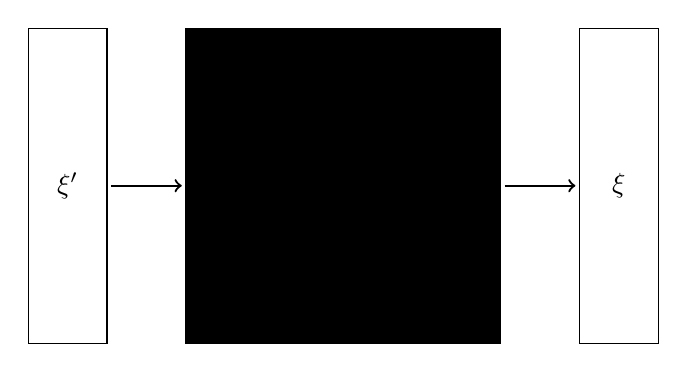
\begin{tikzpicture}
    \draw (0,0) rectangle (1,4);
    \node at (0.5,2) {$\xi^\prime$};
    \draw[thick, ->] (1.05,2) --(1.95,2);

    \filldraw[fill=\fillColor, draw=black] (2,0) rectangle (6,4);
    \node[align=center] at (4,2) {Autoassociative\\Memory};
    
    \draw (7,0) rectangle (8,4);
    \node at (7.5,2) {$\xi$};
    \draw[thick, ->] (6.05,2) --(6.95,2);
\end{tikzpicture}
\end{center}

% \only<1>{
% \begin{center}
% \begin{tikzpicture}
%     \draw (0,0) rectangle (1,4);
%     \node at (0.5,2) {$\xi$};
%     \draw[thick, ->] (1.05,2) --(1.95,2);

%     \filldraw[fill=\fillColor, draw=black] (2,0) rectangle (6,4);
%     \node[align=center] at (4,2) {Autoassociative\\Memory};
    
%     \draw (7,0) rectangle (8,4);
%     \node at (7.5,2) {$\xi$};
%     \draw[thick, ->] (6.05,2) --(6.95,2);
% \end{tikzpicture}
% \end{center}
% }

% \only<2>{
% \begin{center}
%     \begin{tikzpicture}
%         \draw (0,0) rectangle (1,4);
%         \node at (0.5,2) {$\xi$};
%         \draw[thick, ->] (1.05,2) --(1.95,2);
    
%         \filldraw[fill=\fillColor, draw=black] (2,0) -- (4,1.5) -- (4,2.5) --(2,4) -- (2,0);
%         \filldraw[fill=\fillColor, draw=black] (4,1.5) -- (4,2.5) -- (6,4) -- (6,0) -- (4, 1.5);
        
%         \draw (7,0) rectangle (8,4);
%         \node at (7.5,2) {$\xi$};
%         \draw[thick, ->] (6.05,2) --(6.95,2);
%     \end{tikzpicture}
% \end{center}
% }

% \only<3>{
% \begin{center}
%     \begin{tikzpicture}
%         \draw (0,0) rectangle (1,4);
%         \node at (0.5,2) {$\xi$};

%         \draw[thick, ->] (1.05,2) --(6.95,2);
        
%         \draw (7,0) rectangle (8,4);
%         \node at (7.5,2) {$\xi$};
%     \end{tikzpicture}
% \end{center}
% }

% \only<4>{
% \begin{center}
% \begin{tikzpicture}
%     \draw (0,0) rectangle (1,4);
%     \node at (0.5,2) {$\xi^\prime$};
%     \draw[thick, ->] (1.05,2) --(1.95,2);

%     \filldraw[fill=\fillColor, draw=black] (2,0) rectangle (6,4);
%     \node[align=center] at (4,2) {Autoassociative\\Memory};
    
%     \draw (7,0) rectangle (8,4);
%     \node at (7.5,2) {$\xi$};
%     \draw[thick, ->] (6.05,2) --(6.95,2);
% \end{tikzpicture}
% \end{center}
% }
    
\end{frame}

% --------------------------------------------------------------------------------

\subsection{Classical Hopfield Network} 

\begin{frame}
	
    \frametitle{Classical Hopfield Network}
    \begin{columns}[c]
        \column{.6\textwidth}
        \begin{itemize}
            \item Association by Hebbian learning.
            \begin{itemize}
                \item Biological inspiration.
                \item Easy to analyze.
            \end{itemize}
            \item Relax by matrix multiplication.
            \begin{itemize}
                \item Mean field approximation.
                \item Nonlinearity keeps states in bipolar domain.
                \item Energy guaranteed to achieve a minima (under sensible conditions).
            \end{itemize}
        \end{itemize}

        \column{.4\textwidth}
        % TODO Classical Hopfield Image
        \begin{align}
            W &= \sum_{k} \xi_k \otimes \xi_k \\
            \xi_{t+1} &= \text{ Sign}\left( W \cdot \xi_{t} \right) \\
            E \left( \xi \right) &= -\frac{1}{2} \xi^T W \xi
        \end{align}
    \end{columns}
\end{frame}

% --------------------------------------------------------------------------------

\subsection{Modern Hopfield Network} 

\begin{frame}
	
    \frametitle{Modern Hopfield Network}
    \begin{columns}[c]
        \column{.6\textwidth}
        \begin{itemize}
            \item Classical energy wells are too shallow.          
        \end{itemize}
        
        

        \column{.4\textwidth}
        \only<1>{
            \begin{figure}[h]
                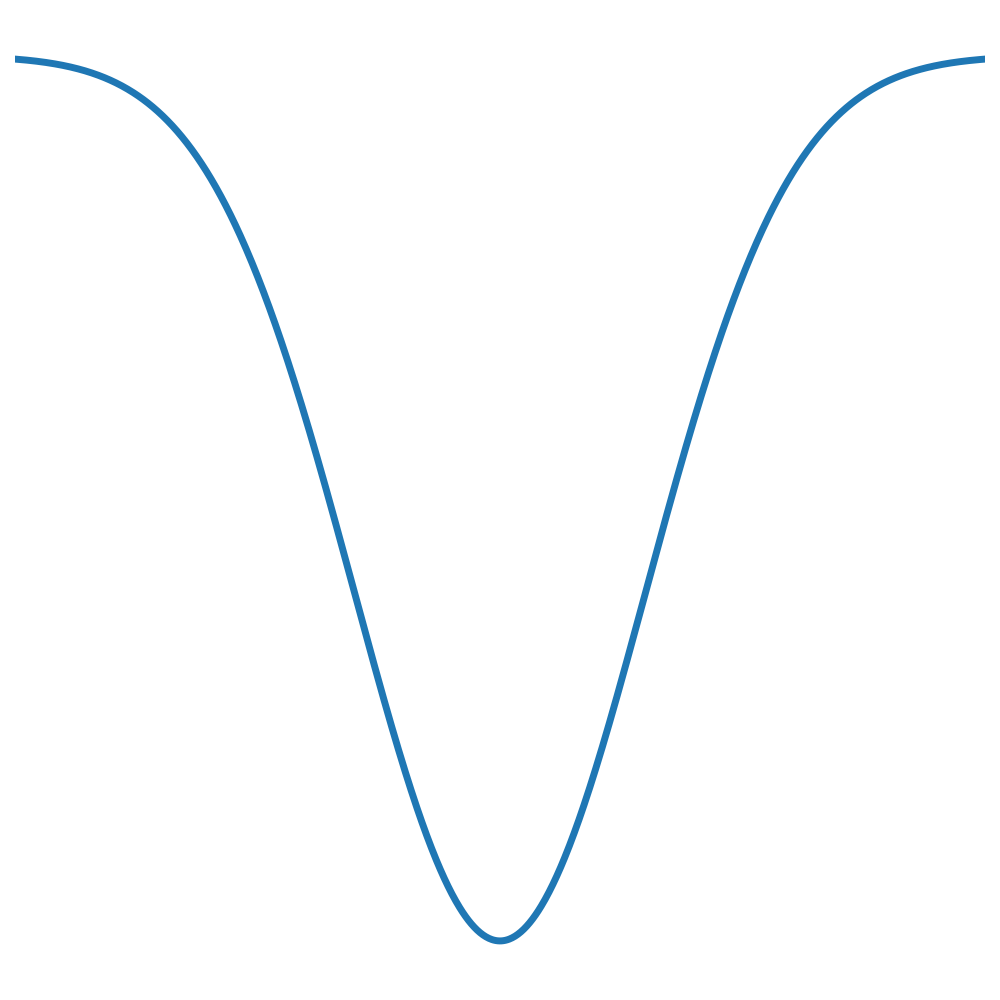
\includegraphics[width=\textwidth]{images/introduction_energywell01.png}
            \end{figure}
        }
        \only<2>{
            \begin{figure}[h]
                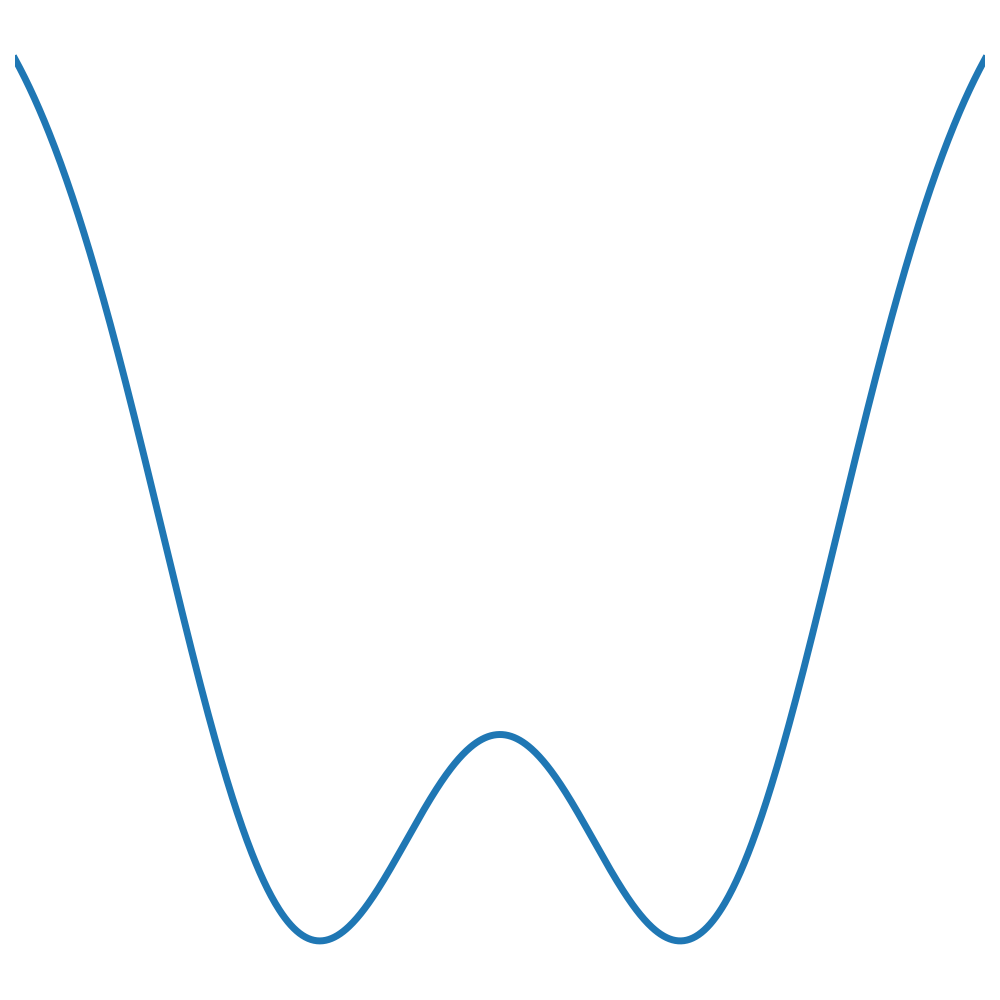
\includegraphics[width=\textwidth]{images/introduction_energywell02.png}
            \end{figure}
        }
        
    \end{columns}
\end{frame}

% --------------------------------------------------------------------------------

\begin{frame}
    \frametitle{Modern Hopfield Network}
    \begin{columns}[c]
        \column{.6\textwidth}
        \begin{itemize}
            \item Key trick: Replace quadratic energy with general polynomial.
            \begin{itemize}
                \item Heck, anything with a vaguely polynomial shape.
            \end{itemize}
        \end{itemize}

        \begin{align*}
            f_n\left( x \right) &= x^n \\
            f_n\left( x \right) &= \begin{cases}
                x^n \; \text{if } x\geq0 \\
                0 \; \text{if } x<0
            \end{cases} \\
            f_n\left( x \right) &= \begin{cases}
                x^n \; \text{if } x\geq0 \\
                -\epsilon x \; \text{if } x<0
            \end{cases}
        \end{align*}

        \column{.4\textwidth}
        \begin{figure}[h]
            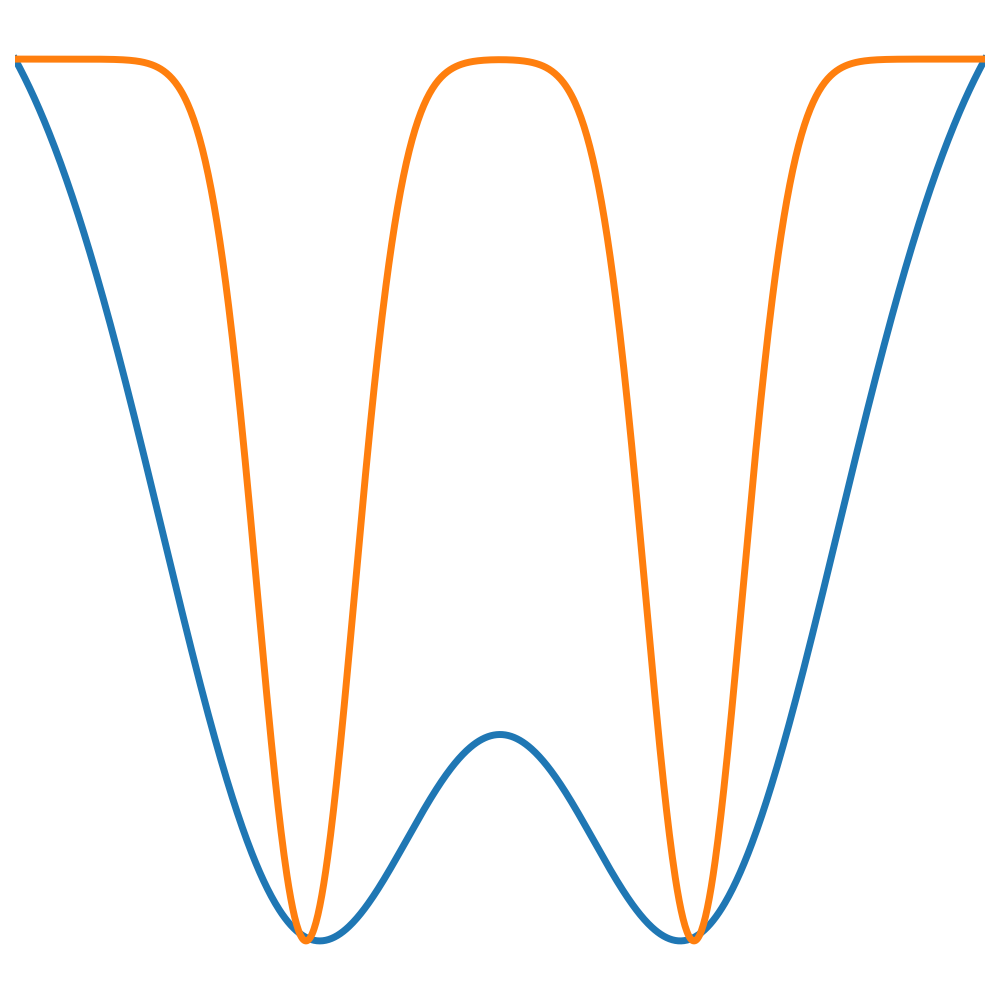
\includegraphics[width=\textwidth]{images/introduction_energywell03.png}
        \end{figure}
    \end{columns}
\end{frame}

% --------------------------------------------------------------------------------

\begin{frame}[t]
	
    \frametitle{Modern Hopfield Network}
    
    \begin{block}{\(n\) -- The Interaction Vertex}
        \begin{itemize}
            \item Controls the range of influence that memories have.
            \item However, also radically alters the network architecture.
        \end{itemize}
    \end{block}

        \only<2>{
            Memory matrix replaced by list of memory states -- vectors of same dimension as data.
            
            \begin{center}
                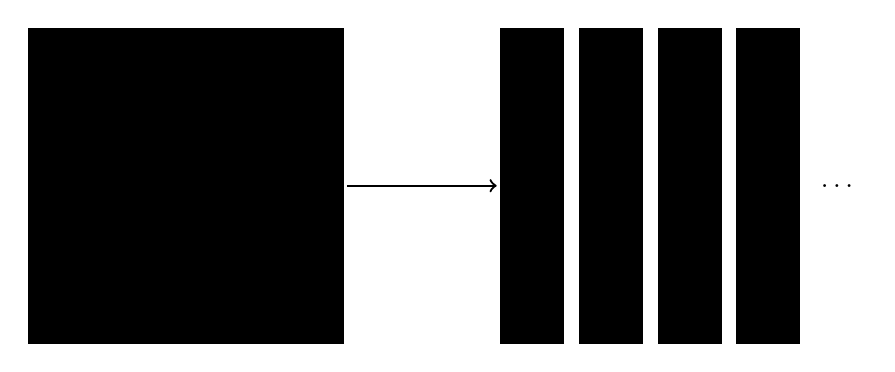
\begin{tikzpicture}
                    \filldraw[fill=\fillColor, draw=black] (0,0) rectangle (4,4);
                    \node at (2,2) {$\xi \otimes \xi$};
                    
                    \draw[thick, ->] (4.05, 2) -- (5.95, 2);
                    \filldraw[fill=\fillColor, draw=black] (6,0) rectangle (6.8,4);
                    \node at (6.4, 2) {$\zeta_0$};
                    \filldraw[fill=\fillColor, draw=black] (7,0) rectangle (7.8,4);
                    \node at (7.4, 2) {$\zeta_1$};
                    \filldraw[fill=\fillColor, draw=black] (8,0) rectangle (8.8,4);
                    \node at (8.4, 2) {$\zeta_2$};
                    \filldraw[fill=\fillColor, draw=black] (9,0) rectangle (9.8,4);
                    \node at (9.4, 2) {$\zeta_3$};
                    \node at (10.3, 2) {\dots};
                \end{tikzpicture}
            \end{center}
        }
        
        \only<3>{
            Relaxation no longer uses mean field -- now a contrastive difference.
            \begin{itemize}
                \item Negative energy no longer means ``stable'' -- the energy \textit{difference} between a neuron clamped on and off indicates stability.
            \end{itemize}

            \begin{center}
                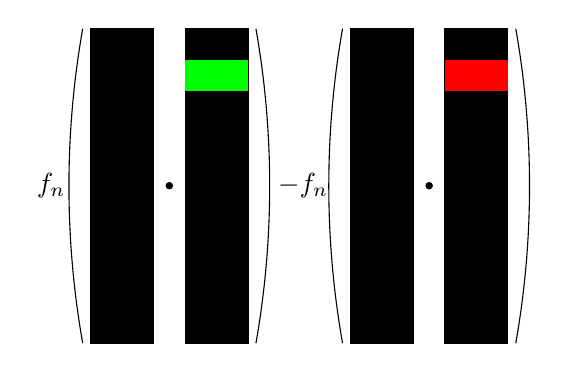
\begin{tikzpicture}
                    \node at (-0.5, 2) {$f_n$};
                    \draw (-0.1, 0) arc (190:170:11.5);
                    \filldraw[fill=\fillColor, draw=black] (0,0) rectangle (0.8,4);
                    \node at (0.4, 2) {$\zeta$};
                    
                    \filldraw (1, 2) circle (0.04);
                    
                    \filldraw[fill=\fillColor, draw=black] (1.2,0) rectangle (2,4);
                    \fill[fill=green] (1.2,3.2) rectangle (2,3.6);
                    \node at (1.6, 2) {$\xi_{+1}$};
                    \draw (2.1, 0) arc (-10:10:11.5);
                    
                    \node at (2.7, 2) {$- f_n$};
                    \draw (3.2, 0) arc (190:170:11.5);

                    \filldraw[fill=\fillColor, draw=black] (3.3,0) rectangle (4.1,4);
                    \node at (3.7, 2) {$\zeta$};

                    \filldraw (4.3, 2) circle (0.04);
                    
                    \filldraw[fill=\fillColor, draw=black] (4.5,0) rectangle (5.3,4);
                    \fill[fill=red] (4.5,3.2) rectangle (5.3,3.6);
                    \node at (4.9, 2) {$\xi_{-1}$};
                    \draw (5.4, 0) arc (-10:10:11.5);
                \end{tikzpicture}
            \end{center}
            
        }

        \only<4>{
            Learning no longer supports Hebbian -- now requires gradient descent.

            \begin{gather*}
             W = \sum_{k} \xi_k \otimes \xi_k \\
             \text{Loss}\left( \xi \right) = \tanh \left[ \beta \sum_{\mu} \left( f_n \left(\zeta_{\mu, i} + \sum_{j \neq i} \zeta_{\mu, j} \xi_{j} \right) - f_n \left( -\zeta_{\mu, i} + \sum_{j \neq i} \zeta_{\mu, j} \xi_{j} \right) \right) \right]
            \end{gather*}
        }

        % \only<5>{
        %     Learning no longer supports Hebbian -- now requires gradient descent.

        %     \begin{gather*}
        %      W = \sum_{k} \xi_k \otimes \xi_k \\
        %      \text{Loss}\left( \xi \right) = \tanh \left[ \textcolor{red}{\boldsymbol \beta} \sum_{\mu} \left( f_n \left(\zeta_{\mu, i} + \sum_{j \neq i} \zeta_{\mu, j} \xi_{j} \right) - f_n \left( -\zeta_{\mu, i} + \sum_{j \neq i} \zeta_{\mu, j} \xi_{j} \right) \right) \right]
        %     \end{gather*}
        % }
        
    
\end{frame}